\documentclass[draftcls,onecolumn,12pt]{IEEEtran}
\usepackage[utf8]{inputenc}
\usepackage[linesnumbered,lined, algoruled]{algorithm2e}
\usepackage{algorithmic,float}
\usepackage{amsmath}
\usepackage{amsthm}
\usepackage{amsfonts}
\usepackage{amssymb}
\usepackage{bm,array}
\usepackage{color,soul}
%\usepackage{epstopdf}
\usepackage[acronym,shortcuts]{glossaries}
\usepackage{graphicx}
\usepackage{graphics}
\usepackage[inline]{enumitem}
\makeglossaries
%%% Glossaries/Acronyms


\newacronym{auc}{AUC}{area under the curve}
\newacronym{bs}{BS}{base station}
\newacronym{ce}{CE}{Cross Entropy}
\newacronym{kl}{K-L}{Kullback-Leibler}
\newacronym{ls}{LS}{least-squares}
\newacronym{llr}{LLR}{log likelihood-ratio}
\newacronym{los}{LOS}{line of sight}
\newacronym{lssvm}{LS-SVM}{least squares SVM}
\newacronym{ml}{ML}{Machine Learning}
\newacronym{mlp}{MLP}{multy-layer perceptron}
\newacronym{mse}{MSE}{Mean Squared Error}
\newacronym[\glslongpluralkey={neural networks}]{nn}{NN}{Neural Network}
\newacronym{np}{N-P}{Neyman-Pearson}
\newacronym{pdf}{PDF}{probability distribution function}
\newacronym{pso}{PSO}{particle swarm optimization}
\newacronym{rnn}{RNN}{replicator neural network}
\newacronym{roc}{ROC}{receiver operating characteristic}
\newacronym{rss}{RSS}{received signal strength}
\newacronym[\glslongpluralkey={support vector machines}]{svm}{SVM}{support vector machine}
\newacronym{ue}{UE}{user equipment}





\newcommand{\ie}{i.e., }
\newcommand{\wrt}{w.r.t. }
\newcommand{\Exp}[1]{\mathbb{E}\left[#1\right]}
\newcommand{\ai}{\mathbf{a}^{(i)}}
\newcommand{\A}[1]{\mathcal{A}_#1}

\DeclareMathOperator{\sign}{sign}
\DeclareMathOperator{\E}{E}
\newtheorem{theorem}{Theorem}
\newtheorem{lemma}{Lemma}

\title{Machine learning approaches for position and user authentication in wireless systems}
\author{ }
\date{}


%\usepackage[autostyle]{csquotes}
\usepackage[backend=biber,style=ieee]{biblatex}
\bibliography{bibliography}


\begin{document}


\maketitle

\sloppy

\begin{abstract}
Physical layer authentication has been proposed as an effective alternative scheme to traditional upper layer-based techniques, such as cryptography, in order to provide a secure authentication scheme. In this paper, we exploit the area specific attenuation values to perform location-based authentication, i.e. granting access to the network only to users located in a pre-defined area. We first exploit the \ac{np} optimal criterion to formulate the problem as hypothesis testing. Secondly, we implement the authentication system by exploiting to \ac{ml} techinques, namely the \acp{nn} and the \ac{svm}. We then show how the output of the \ac{nn} trained with two different loss functions, namely the \ac{mse} and the \ac{ce}, are related to \ac{np} optimal hypothesis testing. The same result has been derived for \ac{svm}. By introducing a realistic channel model we then show that the proposed \ac{nn} implementation of the authentication system is convenient respect to \ac{np}. The problem of network planning is hence addressed and lastly we propose a possible atteck strategy.
\end{abstract}

\begin{IEEEkeywords}
Physical layer security, authentication, neural network, auto-encoder, support vector machine
\end{IEEEkeywords}

\glsresetall

\section{Introduction}
Traditional authentication systems are based on upper-layer techniques such as cryptography. However, as the network latency requirement becomes stricter, the timely sharing of security keys in large and dense networks may not be supported by this type of networks. This is further complicated by the computational cost of key generation and detection. On the other hand, as the computational power of devices grows, the time spent in cracking a digital security key may be remarkably shortened \cite{Wang-16}. Physical layer techniques have been proposed as an alternative to digital key generation. These techniques exploit properties of the communication channel such as the \ac{rss} to distinguish radio transmitters. In this paper, we exploit area specific attenuation values to distinguish between a legitimate and non-legitimate area, implementing in such a way a location-based authentication system.

Traditional detection systems are based on \ac{np} lemma which rejects a hypothesis in favor of the other based on the comparison of the likelihood ratio with a suitably chosen threshold value. An example application of this criterion is \cite{Baracca-12}, where the \ac{np} framework has been exploited to implement an authentication system suited for multiple wiretap channels with correlated fading. A generalization of the \ac{np} framework is presented in \cite{Xiao-09}, where physical layer authentication is performed over a Rayleigh fading channels and detection is implemented via generalized likelihood ratio test. A further example is \cite{Pan-17}, where \ac{ml} algorithms have been exploited in order to find the best threshold needed for hypothesis testing.

However, the knowledge of the channel statistics as well as its model may not be available. In this context, the computation of the likelihood functions needed for hypothesis testing can be estimated by the available data but may not be accurate. \ac{ml} techniques have been introduced as an alternative method to perform user authentication without requiring prior knowledge of the channel statistics. This issue has been tackled by \cite{xiao-2018}, where no assumption is made on the channel model and logistic regression has been proposed as alternative to hypothesis testing. In \cite{Wang-17}, a feed-forward neural network receives as input the Euclidean distance between successive channels and the Pearson coefficient as feature space to perform authentication. 

Other than \acp{nn}, also \acp{svm} have been used to classify channel features. In \cite{tian2015robust} the objective is to locate the user inside a building and the classification problem is multi-class: one class for each room. In \cite{pei2014channel} instead, the authors describe an authentication scheme in which a learning machine (an \ac{svm} and linear Fisher discriminant analysis) is first trained with channel feature vectors and then used to classify the sender as trusted or malicious. Note that neither \cite{pei2014channel} nor \cite{tian2015robust} analyse performance of their \ac{ml} approaches against the theoretical optimum \ac{np} criterion, which we investigate in this work.

In this paper, we compare the performance of the authentication system based on \ac{np} optimality criterion, henceforth referred to as \ac{np} detector, with \ac{ml} based approaches. In particular, we investigate the performance of the \ac{ml}-based authentication systems implemented via \ac{nn} and via \ac{svm}. We consider two different \ac{nn} architectures: the multi-layer perceptron and the auto-encoder. For the multi-layer perceptron, we investigate two loss functions: the \ac{ce} and the \ac{mse}. We show that both loss functions guarantee the same performance of the optimal \ac{np} detector in terms of true positive and false negative rate. Further details about the architectures and the training objective function will be discussed in section \ref{sec:nn}.

In section \ref{sec:auto} we consider the problem of performing hypothesis testing when samples from one of the two classes are available and no information on the other class can be obtained. The auto-encoder \ac{nn} is proposed as solution for this problem.

In section \ref{sec:svm}, we introduce the \ac{svm} and we show how it can be exploited to implement an authentication system. Furthermore, we show that the output of such a system is related to the \ac{np} lemma.

In sections \ref{sec:res_los} and \ref{sec:res_nLos} we confirm via numerical results the theoretical parts of the previous section and investigate the performance of the different implementations of the authentication system.

In section \ref{sec:bsPos}, we consider the problem of network planning, i.e., find the optimal positions of the \acp{bs} needed to implement the authentication system. We show that the \ac{nn} can be exploited in the optimization procedure.

The contribution of this paper can be summarized as follows:
\begin{itemize}
    \item We propose an implementation of a physical layer-based location authentication system which exploits \ac{ml} techniques to perform hypothesis testing;
    \item We show that the performance obtained with this \ac{ml} techniques are optimal in a \ac{np} sense;
    \item We compare different \ac{ml} techniques and show how these can be exploited to implement different levels of the authentication system, from the planning of the network to authentication and attacks.
\end{itemize}

The following notation will be used throughout the paper: bold letters $\bm{x}$ refer to vectors, whereas capital bold letters $\bm{H}$ refer to matrices, $\mathbb{E}[]$ denotes the expected value, $e_i$ denotes the all zero vector except for component $i$ which is equal to $1$ and $(\cdot)^T$ denotes the transpose.

\section{System Model}
We consider a cellular system with $N_{\rm BS}$ \acp{bs} covering a region $\mathcal{A}$ over a plane. We propose a location authentication system able to determine if a \ac{ue} is transmitting from within an {\em authorized} sub-region $\mathcal{A}_0$ of the region$\mathcal{A}$. The authentication process exploits the features of the channel between the \ac{ue} and the \acp{bs}, and in particular the location dependency of these features, that allow to distinguish between a transmission from the region $\mathcal{A_0}$ and a transmission from the complementary region $\mathcal{A}_1=\mathcal{A} \setminus \mathcal{A}_0$. Among the various features (e.g. power, impulse response, phase offset) we consider here a narrowband transmission and we focus on the power received by the \acp{bs} upon \ac{ue} transmission.

In details, the location authentication procedure encompasses two phases. In the first phase ( authentication identification) the \ac{ue} transmits a training signal ( known at the \acs{bs}) from various points within region $\mathcal{A}_0$, and the \acp{bs} estimate the attenuation incurred by the transmission and store them in association with $\mathcal{A}_0$. In this phase some external authentication technique must be used to ensure that the \ac{ue} is in region $\mathcal{A}_0$. Similarly the \ac{ue} transmits a training signal from the complementary area $\mathcal{A}_1$ and the \acp{bs} store the attenuations, associating them to $\mathcal{A}_1$.

In the second phase (authentication verification) the \ac{ue} transmits a known training sequence from any points in $\mathcal{A}$, and the \acp{bs} must decide whether the \ac{ue} is in region $\mathcal{A}_0$ or $\mathcal{A}_1$.

\subsection{Channel model}

\Ac{bs} $n$, $n=1,...,N_{\rm bs}$, is located in position $\bm{x}_{\rm bs}^{(n)} =(X_{\rm bs}^{(n)},Y_{\rm bs}^{(n)})$. For a \ac{ue} located at $\bm{x}_{\rm ue}=(X_u,Y_u)$, its distance from the \ac{bs} is
\begin{equation}
    L(\bm{x}_{\rm ue},\bm{x}_{\rm bs}^{(n)}) = \sqrt{(X_{\rm bs}^{(n)}-X_u)^2+(Y_{\rm bs}^{(n)}-Y_u)^2}.
\end{equation}
When a \ac{ue} transmits with power $P_{\rm tx}$, the received power at the $n^{\rm th}$ \ac{bs} is
\begin{equation}
    P_{\rm rc}^n[dB]= P_{\rm tx}[dB] -  a^{(n)}[dB],
\end{equation}
where $a^{(n)}$ is the attenuation incurred by the transmitted signal to \ac{bs} $n$. The attenuation coefficient includes th effects of path-loss, shadowing and fading, i.e.
\begin{equation}
    \sqrt{a^{(n)}} \sim \mathcal{N}\left(0,\sigma_{a,n}^2\right),
\end{equation}
where $\sigma_{a,n}^2=P_{\ell}^{(n)}-4.34s$ (\hl{citare}), $P_{\ell}^{(n)}$ is the path-loss coefficient and $s \sim \mathcal{N}(0,\sigma_s^2)$ is the shadowing component. For the path-loss we consider two scenarios: \ac{los} and non-\ac{los}.

For a \ac{los} link the path loss coefficinet in dB is modelled as
\begin{equation}\label{eq:los}
    P_{\rm LOS,dB}^{(n)} = 20\log_{10}\left(\frac{f 4\pi L(\bm{x}_{\rm ue},\bm{x}_{\rm bs}^{(n)})}{c}\right),
\end{equation}
where $f$ is the carrier frequency and $c$ is the speed of light.

For a  non-\ac{los} link the path loss coefficient in dB is defined as
\begin{equation}
    P_{\rm non-LOS,dB}^{(n)} = 40\log10\left (\frac{L(\bm{x}_{\rm ue},\bm{x}_{\rm bs}^{(n)})}{10^3}\right ) + 21\log10\left(\frac{f}{10^6}\right) + 80.
\end{equation}

We assume that fading and shadowing are time-invariant while fading is time dependent. The shadowing $s$ depends on positions $\bm{x}_{\rm ue}$ and $\bm{x}_{\rm bs}^{(n)}$ and is correlated at different \ac{ue} and \ac{bs} positions. \hl{aggiungere info}

\subsection{Decision rule with known statistics}\label{sec:auth}
The authentication problem has a straightforward formulation as an hypothesis test. Let us define the two hypothesis: $\mathcal{H}_0$: the \ac{ue} is transmitting from area $\mathcal{A}_0$; $\mathcal{H}_1$: the \ac{ue} is transmitting from area $\mathcal{A}_1$.

Given the attenuation vector $\bm{a}$ we want to determine which of the two hypothesis is more likely to be true in order to implement the aforementioned authentication system. However due to the random nature of the channel (including fading) a given estimated authentication vector $\bm{a}$ can not be associated univocally to one of the two regions. Instead, we indicate with $p(\bm{a}|\mathcal{H}_i)$ the probability of estimating the vector $\bm{a}$ given that hypothesis $\mathcal{H}_i$ is verified (i.e., the \ac{ue} is in region $\mathcal{A}_i$).
Assuming that these conditional distributions are known we can compute the \ac{llr}
\begin{equation}\label{eq:lr}
    \mathcal{L}^{(\bm{a})}=\log\left(\frac{p(\bm{a}|\mathcal{H}_0)}{p(\bm{a}|\mathcal{H}_1)}\right).
\end{equation}
According to the \ac{np} lemma, the most powerful test is obtained by comparing $\mathcal{L}^{(\bm{a})}$ with a threshold value $\Lambda$ i.e., deciding for hypothesis $\mathcal{H}_1$ if $\mathcal{L}^{(\bm{a})} \le \Lambda$ and for hypothesis $\mathcal{H}_0$ if $\mathcal{L}^{(\bm{a})} > \Lambda$. Let us define two error probabilities: the false alarm probability, i.e. the probability  that a legitimate user is classified as non-legitimate $P_{\rm FA} =P(\hat{\mathcal H} = \mathcal H_1 | \mathcal H_0)$; the mis-detection probability, i.e., the probability that a non-legitimate user is classified as legitimate, $P_{\rm MD}=P(\hat{\mathcal H} = \mathcal H_0 | \mathcal H_1)$. The \ac{np} lemma ensures that,for a given false alarm probability, the minimum mis-detection probability is obtained comparing $\mathcal{L}^{(\bm{a})}$ with $\Lambda$, where $\Lambda$is chosen according to the desired false-alarm probability.

Since in practice the statistics $p(\bm{a}|\mathcal{H}_i)$ are not available, we propose to use a machine-learning approach to perform the authentication. To this end we briefly describe here the \ac{nn} and the \ac{svm} that will be used in the next sections.

\subsection{Neural networks}\label{sec:nn}

A \ac{nn} is a function of the type $\mathbb{R}^N \to \mathbb{R}^O$ which maps a set of $N$ real values into $O$ real values. A \ac{nn} processes the input in stages, named layers, where the output of one layer is the input of the next layer. For a \ac{nn} with $L-1$ layers the first layer (layer $0$) is denoted input layer, the last layer (layer $L-1$) is denoted output layer and the other layers are denoted as hidden layers. This architecture is also known as \ac{mlp}

Layer $L-1$ has $N^{(\ell-1)}$ outputs obtained by processing the inputs with $N^{(\ell-1)}$ functions named neurons. The output of the $n^{\rm th}$ neuron of the $\ell^{\rm th}$ layer is
\begin{equation}\label{eq:nonLin}
y_n^{(\ell)} = \psi\left( \bm{w}_n^{(\ell -1)}\bm{y}^{(\ell-1)}+b_n^{(\ell)} \right),
\end{equation}
i.e., a mapping via an activation function $\psi$ of the weighted linear combination with weights $\bm{w}_n^{(\ell -1)}\in \mathbb{R}^{1\times N^{(\ell-1)}}$ of the outputs $\bm{y}^{(\ell-1)} \in \mathbb{R}^{N^{(\ell-1)} \times 1 }$ of the previous layer plus a bias $b_n^{(\ell)} \in \mathbb{R}^{N^{(\ell-1)} \times 1 }$. The \ac{nn} input is $\bm{y}^{(0)}$ while its output is $\bm{y}^{(L-1)}$. The activation function of the input layer is the identity function.

The activation function of the hidden layers is the sigmoid function
\begin{equation}
\psi^{(\ell)}(x) = \frac{1}{1-e^{-x}},
\end{equation}
whereas the activation function of the output layer is 
\begin{equation}
\psi^{(L-1)}(x)=\tanh^{-1}(x) = \frac{1}{2} \left( \frac{1+x}{1-x} \right).
\end{equation}


The vectors $\bm{w}_n^{(\ell)}$ and the scalars $b_n^{(\ell)}$ must be properly chosen for the desired purposes of the \ac{nn}.

Since the output of the neural network $y^{(L-1)}$ is a continuous value in ${-1,1}$, in order to perform classification, a suitable threshold value $\lambda$ must be chosen, such that the input vector $\bm{y}^{(0)}$ is classified as
$\mathcal{H}_0$ if $\bm{y}^{(L-1)} > \lambda$ and as $\mathcal{H}_1$ if $\bm{y}^{(L-1)} \le \lambda$.


In the next sections we investigate the effects of training the \ac{mlp} with two different loss functions: the \ac{mse} and the \ac{ce}.
\subsection{Support Vector Machine}\label{sec:svm}
A \ac{svm} \cite{Bishop2006} is a supervised learning model that can be used for classification and regression. We focus here on binary classification, \ie given the input vector $\bm{y}^{(0)} \in \mathbb{R}^N$ the \ac{svm} returns $\hat{t} = 1$ if $\bm{y}^{(0)}$ belongs to class 0 whereas $\hat{t}=-1$ if $\bm{y}^{(0)}$ belongs to class 1. It comprises the function $\tilde{t}: \mathbb{R}^N \to \mathbb{R}$ defined by
\begin{equation}
\label{eq:svm}
\tilde{t} = \mathbf{w}^T \phi (\mathbf{a}^{(i)}) + b,
\end{equation}
where $\phi: \mathbb{R}^N \to \mathbb{R}^K$ is a feature-space transformation function, $\mathbf{w} \in \mathbb{R}^K$ is the weight vector and $b$ is a bias parameter, and the decision function
\begin{equation}
\label{eq:cases}
\hat{t} = 
\begin{cases}
+1 \quad \tilde{t}  \geq \gamma^* \\
-1 \quad \tilde{t}  < \gamma^*,
\end{cases}		
\end{equation} 
where $\gamma^*$ is a fixed threshold and controls false alarm and miss detection probabilities. Note that in the classical \ac{svm} formulation we have $\gamma^* = 0$.

While typically the feature-space transformation function is fixed, the vector $\mathbf{w}$ must be properly chosen to perform the desired classification
\section{Authentication by machine learning approaches}
The Neyman Pearson approach requires the knowledge of the conditional \ac{pdf} of the pbserved channel feature. When these are not available, as typically, occurs in practical systems, we can resort to \ac{ml} approaches. Note that these solutions do not explicitly evaluate the \ac{pdf} to compute then the \ac{llr}, rather implement directly the primitive by which the decision is taken.

In this Section we \begin{enumerate*}[label=\alph*)]
\item a describe how to learn the decision function with both \ac{nn} and \ac{svm} and \item show that in asymptotic conditions (infinite training) the \ac{nn} and \ac{svm} functions approximate the Neyman-Pearson optimal \ac{llr} function.
\end{enumerate*}

In this Section we assume that the authentication system has access to both regions $\mathcal{A}_0$ and $\mathcal{A}_1$ and that during the authentication phase $S$ attenuation vectors $\ai, \ i=1,\dots S$, are collected, belonging to both regions. For each vector $\ai$ we define the identification function $t_i = -1$ if $\ai$ was obtained using a transmitter in region $\mathcal{A}_0$ and $t_i = 1$ if the transmitter was in region $\mathcal{A}_1$.

We consider two learning strategies (based on the \ac{mse} and \ac{ce} for \ac{nn} \hl{Citare NN} and one learning strategy (the \ac{ls} approach) for \ac{svm} \cite{Suykens1999}.


\subsection{ MSE training}
Let us define as $\tilde{\bm{y}}_{\rm MSE}$ the vector of the output values of the \ac{mlp}, whose $i^{\rm th}$ component is the output of the \ac{mlp} obtained with the $i^{\rm th}$ training vector, and as $\bm{y}_{MSE}$ the vector of the labels of the training vectors. The \ac{mlp} training is performed via gradient descent minimizing the \ac{mse}, defined as
\begin{equation}
MSE = \mathbb{E}[||\tilde{\bm{y}}_{\rm MSE}-\bm{y}_{\rm MSE}||^2].
\end{equation}

We now prove the connection of \ac{mse} training with the \ac{np} theorem.
\begin{theorem}
\label{th:nn_np}
Consider a \ac{nn} with perfect training and a sufficient number of parameters such that training reaches a global minimum. Then the classificator obtained by training the \ac{nn} via \ac{mse} is equivalent to the classificator obtained via \ac{np} lemma.
\end{theorem}
\begin{proof}
It has been shown in \cite{Ruck-90} that a \ac{nn} trained via \ac{mse} implements a function that is the minimum \ac{mse} approximation of the Bayes optimal discriminant function
\begin{equation}\label{eq:bayesDisc}
g_0(\bm{a}) = \mathbb{P}(\mathcal{H}_0|\bm{a}) - \mathbb{P}(\mathcal{H}_1|\bm{a}).
\end{equation} 
By recalling that $\mathbb{P}(x|y)=\mathbb{P}(y|x)\mathbb{P}(x)/\mathbb{P}(y)$ we can write
\begin{equation}
g_0(\bm{a}) = \frac{{\mathbb P}(\bm{a}|\mathcal H_0){\mathbb P}(\mathcal H_0) - {\mathbb P}(\bm{a}|\mathcal H_1){\mathbb P}(\mathcal H_1)}{\mathbb P(\bm{a})},
\end{equation}
which in turn can be written as
\begin{equation}
g_0(\bm{a}) = \frac{{\mathbb P}(\bm{a}|\mathcal H_0){\mathbb P}(\mathcal H_0) - {\mathbb P}(\bm{a}|\mathcal H_1){\mathbb P}(\mathcal H_1)}{{\mathbb P}(\bm{a}|\mathcal H_0){\mathbb P}(\mathcal H_0) + {\mathbb P}(\bm{a}|\mathcal H_1){\mathbb P}(\mathcal H_1)}.
\end{equation}
By imposing a threshold $\lambda$ on $g_0(\bm{a})$ and reorganizing we obtain
\begin{equation}
\frac{{\mathbb P}(\bm{a}|\mathcal H_0)}{{\mathbb P}(\bm{a}|\mathcal H_1)}>   \frac{{\mathbb P}(\mathcal H_1)}{{\mathbb P}(\mathcal H_0)} \frac{1 + \lambda}{1-\lambda} = \lambda^*,
\end{equation}
which is equivalent to the \ac{np} criterion.
\end{proof}

\subsection{CE training}
In this case the \ac{nn} training is performed via gradient descent minimizing the \ac{ce} defined as
\begin{equation}\label{eq:ce}
CE = -\sum_{i=1}^{S}\left(\tilde{y}_i^{\rm CE}\log\left(y_i^{\rm CE}\right)+\left(1-\tilde{y}_i^{\rm CE}\right)\log\left(1-y_i^{\rm CE}\right) \right).
\end{equation}
When training is performed with \ac{ce} loss function the output of the \ac{nn} is the minimum \ac{mse} approximation of the probability $\mathbb{P}(\mathcal{H}_0|\bm{a}^{(i)})$ of being in hypothesis $\mathcal{H}_0$ given that the attenuation vector is $\bm{a}^{(i)}$ \cite{Bishop2006}, i.e.,
\begin{equation}
    f(\bm{a}^{(i)},\bm{W}) \approx \mathbb{P}(\mathcal{H}_0|\bm{a}^{(i)}),
\end{equation} 
where $\bm{W}$ is the matrix whose $\ell{\rm th}$ column is obtained by stacking the vector of weights $\bm{w}_n^{(\ell)}$ and bias $b_n^{(\ell)}$ of each neuron of the $\ell{\rm th}$ layer.

We then have the following result
\begin{theorem}
\label{th:nn_np2}
Consider a \ac{nn} with perfect training and a sufficient number of parameters such that the training reaches a global minimum. Then the classificator obtained by training the \ac{nn} via \ac{ce} is equivalent to the classificator obtained via \ac{np} lemma.
\end{theorem}
\begin{proof}
Since we are considering a two class classification problem the probability $\mathbb{P}(\mathcal{H}_1|\bm{a}^{(i)})$, i.e., the probability of being in hypothesis $\mathcal{H}_1$ given that the attenuation vector is $\bm{a}^{(i)}$, is obtained as
\begin{equation}
    \mathbb{P}(\mathcal{H}_1|\bm{a}^{(i)}) = 1- \mathbb{P}(\mathcal{H}_0|\bm{a}^{(i)}).
\end{equation}
By imposing a threshold on the output of the \ac{nn} we obtain
\begin{equation}
    \mathbb{P}(\mathcal{H}_0|\bm{a}^{(i)}) \approx  f(\bm{a}^{(i)},\bm{W}) \gtrapprox \lambda,
\end{equation}
which can be rewritten as
\begin{equation}
    2\mathbb{P}(\mathcal{H}_0|\bm{a}^{(i)})-1 \gtrapprox \hat{\lambda}
\end{equation}
\begin{equation}
    \mathbb{P}(\mathcal{H}_0|\bm{a}^{(i)})-(1-\mathbb{P}(\mathcal{H}_0|\bm{a}^{(i)})) \gtrapprox \hat{\lambda}
\end{equation}
\begin{equation}
    \mathbb{P}(\mathcal{H}_0|\bm{a}^{(i)})-\mathbb{P}(\mathcal{H}_1|\bm{a}^{(i)}) \gtrapprox \hat{\lambda}.
\end{equation}
We hence obtained the same formulation of (\ref{eq:bayesDisc}) and, by following the same steps of the proof of theorem 1 we see that imposing a threshold on the output of the \ac{ce}-trained \ac{nn} is equivalent of performing hypothesis testing with \ac{np} lemma.
\end{proof}


\subsection{Least-Squares approach for \ac{svm}}
For the learning phase of \ac{svm} we consider the \ac{lssvm}, an extension of the \ac{svm} first introduced in \cite{Suykens1999}. In \cite{Yevs} it is shown that  \ac{svm} and \ac{lssvm} are equivalent under mild conditions. The learning in \ac{lssvm} is performed by solving the following optimization problem
\begin{subequations}
	\label{eq:lssvm}
	\begin{equation}
	\label{eq:lssvmOrig}
	\underset{\mathbf{w},e}{\text{min}} \quad f_l(\mathbf{w},e) = \frac{1}{2} \mathbf{w}^T \mathbf{w} + C \frac{1}{2} \sum_{i=1}^S e_i ^2 
	\end{equation}
	\begin{equation}
	\label{eq:stpart}
	\text{subject to}\,  \hat{t}_i[\mathbf{w}^T \phi (\mathbf{a}^{(i)}) + b] = 1- e_i\quad i = 1 ,\dots,S.
	\end{equation}
\end{subequations}

From the constraints in \eqref{eq:lssvm} and the fact that $\hat{t}_i = \pm 1$ we have
\begin{equation}
\label{eq:els}
e_i^2 = (1 - \hat{t}_iy(\mathbf{a}^{(i)}) )^2 = (\hat{t}_i - y(\mathbf{a}^{(i)}))^2,
\end{equation}
that is the squared error between the soft output of the \ac{lssvm} $y(\mathbf{a}^i)$ and the correct training label $\hat{t}_i$. We now prove the equivalence between the \ac{lssvm} and \ac{np} classificators. 

Let us first consider the following lemma that establishes the convergence of the learning phase of \ac{svm}, as the training sample set becomes large.

\begin{lemma}
	\label{lem:lem1}
	For training samples $\bm{a}^{(i)}$ from a finite alphabet $\mathcal A$, taken with a given static probability distribution, for large number of training samples, i.e., as $S \rightarrow \infty$, the vector $\bm{w}$ of the \ac{lssvm} converges in probability to a vector of finite norm $||\mathbf{w}||_2 = \mathbf{w}^T\mathbf{w}$.
\end{lemma}

\begin{proof}
	Given a finite alphabet $\mathcal A = \{\bm{\alpha}_1, \ldots, \bm{\alpha}_M\}$ of $M$ elements for $\bm{a}^{(i)}$, we indicate with $p_{\bm{a}^{(i)},\hat{t}_i}(\bm{\alpha}_j,\hat{t})$, with $\hat{t} \in \{-1,1\}$, the joint probability of input vector $\bm{a}^{(i)}$ and corresponding output $\hat{t}_i$, $i=1, \ldots, S$.
	
	By the Glivenko–Cantelli theorem we have that with probability 1 as $S\rightarrow \infty$ there are $Sp_{\bm{a}^{(i)},\hat{t}_i}(\bm{\alpha}_j,\hat{t})$ training vectors $\bm{\alpha}_j$ with associated true value $\hat{t}$ in any training sequence.
	All these training points will have the same value $e_i$, from (\ref{eq:stpart}), that will appear $Sp_{\bm{a}^{(i)},y_i}(\bm{\alpha}_j,\hat{t})$ times in the sum $\sum_{i=1}^{S} e_i^2$.
	Note that in the training ensemble there could be two equal instances $\mathbf{a}^{(m)}=\mathbf{a}^{(n)}=\bm{\alpha}_j$, but with different labels $\hat{t}_m \neq \hat{t}_n$. Therefore, for $\mathbf{a}^{i}=\bm{\alpha}_j$ we can have two possible values for $e_i$, depending on $y_i$, and we denote them with $e_{j,1}$ and $e_{j,-1}$.
	This translates in only $2M$ \textit{distinct} constraints of the type \eqref{eq:stpart}.
	Asymptotically, for $S \to \infty$, problem (\ref{eq:lssvm}) becomes
	\begin{subequations}
		\label{eq:lssvm22}
		\begin{equation}
		\label{eq:lssvm2}
		\underset{\mathbf{w},e}{\text{min}} \quad f_l(\mathbf{w},e) = \frac{1}{2} \mathbf{w}^T \mathbf{w} + C S \frac{1}{2} \sum_{j=1}^M [p_{\bm{a}^{(i)},\hat{t}_i}(\bm{\alpha}_j,1) e_{j,1}^2 + p_{\bm{a}^{(i)},y_i}(\bm{\alpha}_j,-1) e_{j,-1}^2]  
		\end{equation}
		\begin{equation}
		\label{eq:stpart2}
		\text{subject to}\,  [\mathbf{w}^T \phi (\bm{\alpha}_j) + b] = 1- e_{j,1}\quad j = 1 ,\dots,M.
		\end{equation}
		\begin{equation}
		\label{eq:stpart3}
		\quad  -[\mathbf{w}^T \phi (\bm{\alpha}_j) + b] = 1- e_{j,-1}\quad j = 1 ,\dots,M.
		\end{equation}
	\end{subequations}
	which solution provides the convergence value (in probability) of vector $\bm{w}$. 
	Note that while the original problem \eqref{eq:lssvm} as $S \to \infty$ has infinite constraints, it can be solved by the problem \eqref{eq:lssvm22} that includes a finite number $2M$ of constraints.
	
	We now solve \eqref{eq:lssvm22} with the dual formulation following the same steps used for the \ac{lssvm} in \cite{Suykens1999} with minor modifications. In particular, when building the Lagrangian we need to introduce two sets of multipliers: $v_k$ for \eqref{eq:stpart2} and $u_k$ for \eqref{eq:stpart3}, $k=1,\dots, M$. Then, by deriving with respect to $\mathbf{w}$ and setting to 0, we obtain 
	\begin{equation}
	\label{eq:wSolution}
	\begin{aligned}
	%	\mathbf{w}\mathbf{w}^T =& \sum_{k=1}^{M} \sum_{h=1}^{M} v_k v_h k(\bm{\alpha}_k,\bm{\alpha}_h)	
	%								- \sum_{k=1}^{M} \sum_{h=1}^{M} v_k u_h k(\bm{\alpha}_k,\bm{\alpha}_h)	\\
	%							&	\sum_{k=1}^{M} \sum_{h=1}^{M} u_k u_h k(\bm{\alpha}_k,\bm{\alpha}_h)
	%								- \sum_{k=1}^{M} \sum_{h=1}^{M} u_k v_h k(\bm{\alpha}_k,\bm{\alpha}_h) \\
	\mathbf{w}\mathbf{w}^T =&  \sum_{k=1}^{M} \sum_{h=1}^{M} k(\bm{\alpha}_k,\bm{\alpha}_h) (v_kv_h + u_ku_h -2 v_ku_h),
	\end{aligned}
	\end{equation}
	where we used the fact that the kernel function
	\begin{equation}
	k(\bm{\alpha}_k,\bm{\alpha}_h) \triangleq \phi(\bm{\alpha}_k) \phi(\bm{\alpha}_h)^T
	\end{equation} is symmetric \wrt its inputs. We conclude that $\mathbf{w}$ has a finite norm since the rhs of \eqref{eq:wSolution} is a finite sum.
	
\end{proof}

\begin{theorem}
	\label{th:lsnp}
	Consider a \ac{lssvm} with perfect training, \ie the training reaches a global minimum of $f_l(\mathbf{w},e)$ given an infinite number of training points $\bm{a}^{(i)}$ drawn from the finite alphabet $\mathcal A$. Then the classificator obtained by training the \ac{lssvm} and by thresholding the soft output \eqref{eq:svm} is equivalent, in the \ac{mse} sense, to the classificator obtained via \ac{np} lemma.
\end{theorem}
\begin{proof}
	From \eqref{eq:lssvmOrig} consider
	\begin{equation}
	\label{eq:lssvmDim1}
	\lim_{S \to +\infty} \frac{1}{S} f_l(\mathbf{w},e) =\frac{C}{2} \lim_{S \to +\infty}\frac{1}{S}  \sum_{i=1}^S e^2_i	=\frac{C}{2}\E_t(\mathbf{w},b),
	\end{equation}
	where $\E_t(\mathbf{w},b) = \Exp{\left(y_i - y(\mathbf{a}^{(i)})\right)^2} $ is the expected value carried out \wrt the training points $\mathbf{a}^{(i)}$. 
	The first equality of \eqref{eq:lssvmDim1} comes from Lemma 1: since $\mathbf{w}$ converges to a finite norm, we can write
	\begin{equation}
	\lim_{S\to \infty} \frac{1}{S} \mathbf{w} \mathbf{w}^T 	= 0.
	\end{equation} 
	The last equality comes from the strong law of large numbers. In the limit, the optimization problem \eqref{eq:lssvm} is equivalent to
	\begin{equation}
	\label{eq:lsInf}
	\begin{aligned}
	& \underset{\mathbf{w},b}{\text{min}} & &  \E_t(\mathbf{w},b), & 
	\end{aligned}	
	\end{equation}
	where we dropped the constraints in \eqref{eq:lssvm} by substitution using \eqref{eq:els}. The optimization problem is the same as in the \ac{nn} case and from \cite{Ruck-90} we have that the couple $(\mathbf{w}^*,b^*)$ minimizing \eqref{eq:lsInf} and parametrizing \eqref{eq:svm} is such that
	\begin{equation}
	y(\mathbf{a}^i;\mathbf{w}^*,b^*)  \approx \mathbb{P}(\mathcal{H}_0|\mathbf{a}^{(i)}) - \mathbb{P}(\mathcal{H}_1|\mathbf{a}^{(i)}).
	\end{equation}
	The proof now is the same as in Theorem \ref{th:nn_np}.
\end{proof}

%It is common practice in the literature \cite{Bishop2006,Suykens1999} to work with the dual formulation of the optimization problems \eqref{eq:svmS} to \eqref{eq:lssvm} by constructing the Lagrangian. 
%In the dual formulation objective functions and constraints are expressed as functions of the kernel 
%\begin{equation}
%	\psi(\mathbf{r}_i,\mathbf{r}_j) = \phi (\mathbf{r}_i)^T \phi(\mathbf{r}_j),	
%\end{equation}
%without explicitly defining the function $\phi(\cdot)$. 
%The output of $\phi(\cdot)$ can now be of infinite dimension, like with the radial kernel family
%\begin{equation}
%	\psi(\mathbf{r}_i,\mathbf{r}_j; \sigma) = \exp \left( \frac{|| \mathbf{r}_i - \mathbf{r}_j ||^2}{2\sigma^2} \right).
%\end{equation}
%In this case, Theorem \ref{th:lsnp} holds only if
%\begin{equation}
%	\lim_{S \to +\infty} \frac{1}{S} \mathbf{w}^T \mathbf{w} < +\infty.	
%\end{equation} 
%However, if we let $C \to +\infty$ in \eqref{eq:lssvm}

\section{One-class Classification}
\label{sec:OneClass}

In practice having learning points in both regions $\A{0}$ and $\A{1}$ may be difficult since \begin{enumerate*}[label=\alph*)] \item region $\A{1}$ wider and not necessarily well defined (being simply the complementary region of $\A{0}$) and \item the attacker may use multiple antennas and by beamforming and power allocation can induce attenuation estimates that not necessarily correspond to points in the region $\A{1}$. About point b), we will further discuss attack possibilities in Section \ref{sec:attack}.

Due to inconsistencies of attenuation vector not belonging to region $\A{0}$, we propose here an authentication system that in the identification association (or learning) phase uses only samples obtained from region $\A{0}$. This problem can also be denoted as one-class classification since we know only samples taken from one of the classes of the classifier. We now present solutions implemented with both \ac{nn} and \ac{svm}.
\end{enumerate*} 

\subsection{Replicator neural network}
\label{sec:auto}

In order to solve this problem we exploit a \ac{nn} that implements a \textit{\ac{rnn}}, i.e., a network that is trained to: a) convert high-dimensional inputs to low-dimensional codes in the hidden layer; b) reconstruct the high-dimensional input at the output layer from the low-dimensional codes of the hidden layer \cite{Hinton-2006}.

Consider a set $\mathcal{U}$ and a set of vectors $\mathcal{V} \in \mathcal{U}$. If this vectors are used for training the auto-encoder, each new input vector $\bm{v} \in \mathcal{U}$ is mapped at the output with a small reconstruction error, whereas each input vector $\bm{v} \notin \mathcal{U} $ is mapped at the output with a large reconstruction error.

The capacity of the auto-encoder to replicate only certain values at the output is due to the fact that the hidden layer is able the extract the features of the set $\mathcal{U}$ used for training. This is particularly true when the size of the hidden layer is lower than the size of the input layer, i.e. when $M<N$ \cite{Bourlard-88}.

Consider an \ac{rnn} with three layers, i.e., a size $N$ input layer, a size $M$ hidden layer and a size $N$ output layer.  The function mapping the input layer to the hidden layer is of the form (\ref{eq:nonLin}), whereas the non-linearity is removed when mapping the hidden layer to the output layer. This is due to the fact that the network must reconstruct real values and hence the output shall not be limited in a range of values. 

The $n^{\rm th}$ output $y_n^{(o)}$ of the output layer is obtained from
\begin{equation}
    y_n^{(o)}= \bm{w}_n^{(o)}\bm{y}^{(h)}+b_n^{(h)}
\end{equation}
where $\bm{w}_n^{(o)}$ is the $1\times M$ vector of weights assigned to the $n^{\rm th}$ output, $\bm{y}^{(h)}$ is the $M\times 1$ vector of the outputs of the hidden layer and $b_n^{(h)}$ is the $n^{\rm th}$ bias of the hidden layer.


We here exploit the \ac{rnn} to implement the authentication system described in section \ref{sec:auth}. 

Consider the input attenuation vector $\bm{a}$ and its replicated value $\hat{\bm{a}}$ at the output of the auto-encoder after training.
Let us define the reconstruction error
\begin{equation}\label{eq: rec err}
    \epsilon = \frac{1}{N}\sum_{i=1}^{N}|a_i-\hat{a}_i|^2,
\end{equation}
where $a_i$ denotes the $i^{\rm th}$ component of the vector. The authentication system performs a test comparing the reconstruction error $\epsilon$ with a threshold value $\gamma$ and chooses 
\begin{equation}
\bm{a} \in
\begin{cases}
\mathcal{A}_0 \, \text{if} \, \epsilon < \gamma \\
\mathcal{A}_1 \, \text{if} \, \epsilon \ge \gamma. 
\end{cases}
\end{equation}

\subsection{One-Class Support Vector Machine}
In this section we consider the one-class \ac{svm} as first introduced in \cite{Scholkopf2001estimating}. The one-class \ac{svm} defines the same decision function as in \eqref{eq:cases}, however the training optimization problem is slightly different:
\begin{subequations}
	\label{eq:oneClassSvm}
	\begin{equation}
	\label{eq:oneClass1}
	\underset{\mathbf{w},\psi, b}{\text{min}} \quad f_o(\mathbf{w},\psi, b) \triangleq
	 \frac{1}{2} \mathbf{w}^T \mathbf{w} +  \frac{1}{\nu S} \sum_{i=1}^S \xi_i + b 
	\end{equation}
	\begin{equation}
	\label{eq:oneClassConstr}
	\text{subject to}\, \mathbf{w}^T \phi (\mathbf{a}^{(i)}) + b \geq - \xi_i, \, \xi_i \geq 0,  \quad i = 1,\dots S, 
	\end{equation}
\end{subequations}
where $\nu \in (0,1]$ is a hyper-parameter.
Note that in the one-class case, the bias parameter $b$ appears also in the objective function.


\section{BSs' optimal position}\label{sec:bsPos}
As attenuation maps are different at each \ac{bs} and depend on the surrounding environment in terms of shadowing effects the performance of the authentication system depends on the number of \acp{bs} and their position. In this section we derive an approach to optimally locate \acp{bs} so that the authentication system attains the best performance. 

Consider a sufficiently large training set which is representative of the attenuation vectors measured from both $\mathcal{A}_0$ and $\mathcal{A}_1$. An \ac{mlp} trained with such a set is not likely to find a large number of outliers when tested. In this sense we can say that if a \ac{mlp} attains better performance that another one in the training phase, then it attains better performance also in the testing phase. We hence test different positions for $N_{\rm BS}$ \acp{bs} and, for each one, we train a \ac{mlp} with a sufficient number of training vectors and compute the minimum value obtained by the gradient descent algorithm used for training.

Fig. \ref{fig:mseVSauc} shows the performance obtained with $8$ random positions for $N_{\rm BS}=5$ \acp{bs}. For all curves is reported the minimum \ac{mse} obtained during training and the corresponding \ac{auc} after testing. We see that \ac{mse} values can be divided in ranges, each one corresponding to different values of \ac{auc}. In particular we notice that lower ranges of \ac{mse} correspond to higher values of \ac{auc}. For \acp{mlp} attaining  \ac{mse} values within the same range we must instead also perform testing in order to choose the configuration with better classification performance. Hence, in order to find the optimal configuration we implement an iterative algorithm which, for each configuration, build a training set and trains a \ac{mlp} and updates the position of the \acp{bs} according to the obtained \ac{mse} value. When the difference between the current \ac{mse} value and that obtained at the previous iteration is smaller than a threshold value $\lambda_{\rm diff}$ then a testing set is built and the relative \ac{auc} values are computed. The configuration with higher \ac{auc} is then selected as the optimal one.

\begin{figure}
    \centering
    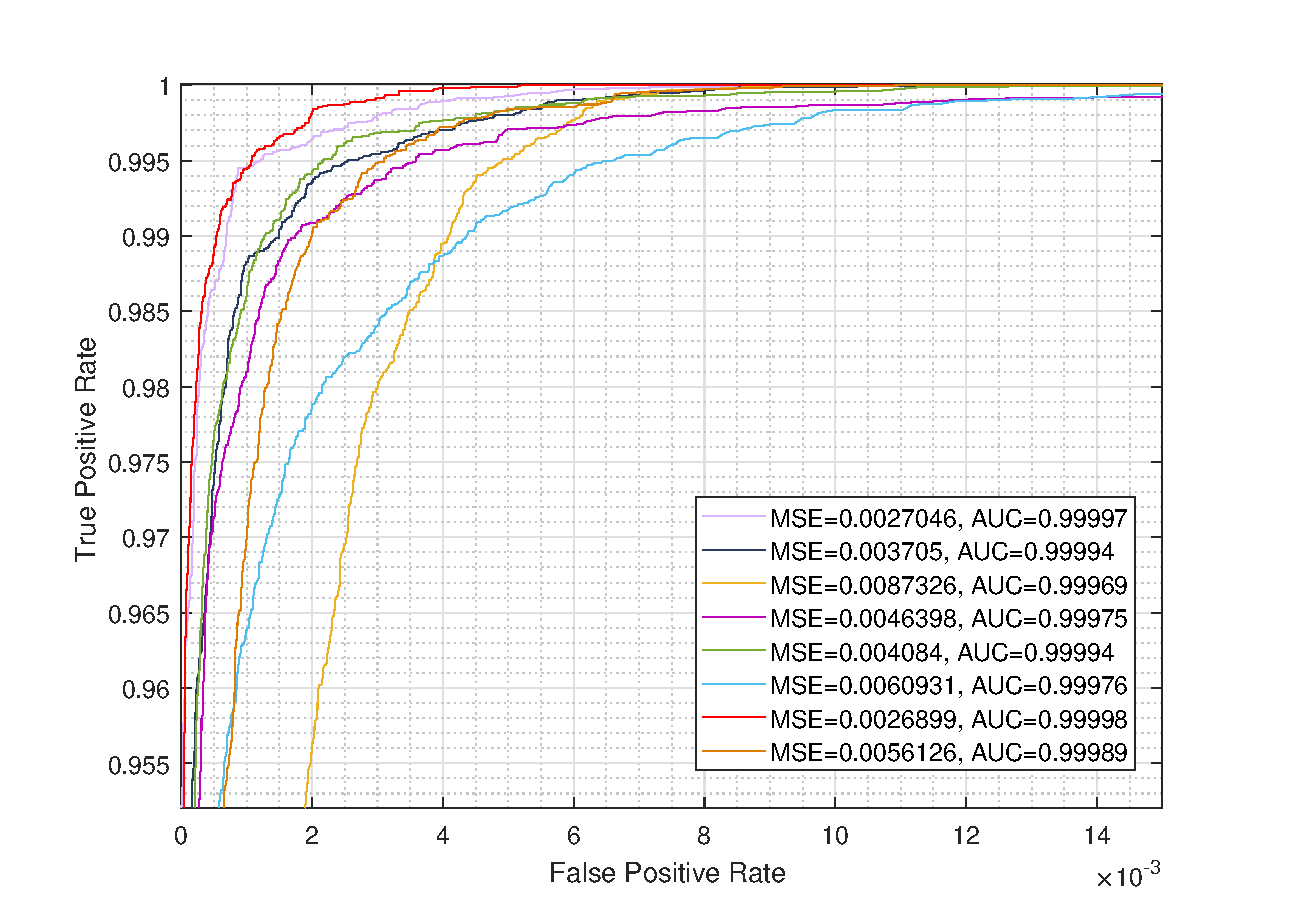
\includegraphics[width=0.5\columnwidth]{mseVSauc.eps}
    \caption{\ac{roc} curves for different BS positions. Lower \ac{mse} are associated to higher \ac{auc}}
    \label{fig:mseVSauc}
\end{figure}

Notice however that the problem is non-convex as the map realization depends on the \acp{bs} position and on a random shadowing and fading realization. Therefore we exploit the \ac{pso} \cite{Kennedy-11}.

\ac{pso} is an iterative optimization algorithm based on social behavior of animals (e.g. birds flocking and fish schools). Consider a particle as a set of positions for the \acp{bs} and consider a total number of $P$ particles. Each one is a possible candidate solution of the optimization problem. Each particle is described by its position $\bm{x}_p$, which is a $N_{\rm BS}$ dimensional vector containing the positions of the \acp{bs} and representing a possible solution, and its velocity $\bm{v}_p$.
Starting from a random initialization of all the particles at each iteration both the positions $\bm{x}_p$ and the velocities $\bm{v}_p$ are updated. Two optimal values are defined in each iteration: the global optimal value found so far by the entire population and a local optimal value for each particle, i.e., the optimal value found by the individual $p$ up to the current iteration. We define as $\bm{o}_g$ the position of the the global optimal values and as $\bm{o}_p$ the position of the optimal value found by particle $p$ at the current iteration.

The position and velocity of the particles are updated at iteration $t$ as
 \begin{equation}\label{eq: v up}
 \bm{v}_p(t) = w\bm{v}_p(t-1)+\phi_1(t)(\bm{o}_p(t-1)-\bm{x}_p(t-1))+\phi_2(t)(\bm{o}_g(t-1)-\bm{x}_p(t-1)), 
 \end{equation}
 \begin{equation}\label{eq: p up}
 \bm{x}_p(t) = \bm{x}_p(t-1) + \bm{v}_p(t),
 \end{equation}
where $w$ is the inertia coefficient and $\phi_1$ and $\phi_2$ are random variables distributed respectively in $[0,c_1]$ and $[0,c_2]$, where $c_1$ and $c_2$ are defined as acceleration constants. The values of the inertia coefficient and of the acceleration constants are the parameters of the \ac{pso} problem. Typical values for this parameters are $w=0.7298$, $c_1=c_2=1.4961$ \cite{Kennedy-11}.

The algorithm steps for \acp{bs} positioning are reported in Algorithm 1. We initialize $P$ particles with random positions for each of the $N_{\rm BS}$ in each particle. For each particle $p$ we then build and train a \ac{nn} and compute the achieved \ac{mse} value MSE$_p^{(0)}$. \ac{pso} is then exploited to iteratively update the position of the particles. Notice that in order to find the best local and global optimal positions \ac{mse} values at the current and previous iterations are compared. If this values are in the same range, i.e., if $|\rm{MSE}_p^{(it-1)}-\rm{MSE}_p^{(it)}|<\lambda_{\rm diff}$ then the \acp{nn}  are also tested and decision is taken based on the \ac{auc} values, otherwise decision is taken based on \ac{mse} values.

\begin{algorithm}[t]
  \algsetup{linenosize=\tiny}
  \scriptsize

 \KwData{ number of particles $P$, $N_{\rm BS}$, $\lambda_{\rm diff}$}
 \KwResult{optimal position }
 Initialization: select random positions for the components of each particle\;
                 build training set for each particle\;
                 build and train a \ac{nn} for each particle and obtain the training performance $\rm{MSE}_p^{(0)}$, $p=1,...,N_p$\;
                 $it = 0$\;

 \Repeat{convergence of particles positions}{
        $it = it + 1$\;
        \For{$p=1,...,P$}{
        update velocity and position vector of particle $p$ via (\ref{eq: v up}) and (\ref{eq: p up})\;
        build a training set\;
        build and test a \ac{nn} and compute $\rm{MSE}_p^{(it)}$\;
        \eIf{$|\rm{MSE}_p^{(it-1)}-\rm{MSE}_p^{(it)}|<\lambda_{\rm diff}$}{
        compute $\rm{AUC}_p^{(it-1)}$ and $\rm{AUC}_p^{(it)}$ for both \acp{nn}\;
        update PSO vectors based on AUC$_p$\;
        
        }{
        update PSO vectors based on MSE$_p$\;
        }
        
        }
      
      }
    
 \caption{BSs positioning algorithm}
\end{algorithm}

The position of the particle that achieves the global minimum \ac{mse} or maximum \ac{auc} at the end of the optimization problem is the best position for the \acp{bs}. Notice that, as the optimization problem is non-convex, solving \ac{pso} is similar to a multi-start  optimization considering $P$ different starting points, which is a standard method used to avoid local minimums. Hence as the number $P$ increases the probability of finding a local solution is reduced.

Notice that the \acp{bs} positioning problem could be solved without implementing a \ac{nn} by mean of computation of the \acp{llr} for the different positions. However we showed in Section \ref{sec:shadow} that when considering multiple \acp{bs} and including shadowing effects the exact computation of the \ac{llr} curve requires more data than those needed for training a \ac{nn}. Hence the proposed solution is effective in terms of both authentication performance and number of needed data.

\section{Attack strategies}
\label{sec:attack}
The proposed techniques can be exploited in order to provide not only an authentication system, but also for implementing an attack strategy. The idea is here to use attenuation values measured from the non-authentic area and to train a \ac{ml} architecture based on these values.

The first architecture we exploit is the \ac{rnn}. The \ac{rnn} is here trained in order to reproduce at the output attenuation vectors measured from the non-authentic area. We propose two attack strategies: a random generation attack and a manifold based attack.

\subsection{Random generation attack}
After that the \ac{rnn} has been trained with attenuation vectors measured from the non-authentic area, only attenuation vectors with the same statistical structure will be reproduced at the output with a reconstruction error $\epsilon$ (\ref{eq: rec err}) lower than $\gamma$. The idea is hence to generate a random attenuation vector $\bm{a}_{\rm test}$ and to feed it to the \ac{rnn}: if the output has a reconstruction error lower than $\gamma$ then $\bm{a}_{\rm test}$ is considered as belonging to the non-authentic area, otherwise it is considered as a possible candidate for a successful attack. This vector is hence tested and, if the attack is not successful, we label it as belonging to the non-authentic area.

As new randomly generated vectors are not successful or have a reconstruction error lower than $\gamma$ we gain information about the structure of the non-authentic area. We hence update the \ac{rnn} training in a mini-batch fashion when a sufficient number of new vectors (good results can be achieved with batch size of $m=3$ or $m=4$ new vectors per update \cite{bengio-12}) is obtained. These vectors are stored in matrix $\bm{A}_{\rm test}$ and when $m$ vectors populate the matrix mini-batch gradient descent is executed on the \ac{rnn} to update its parameters.

The algorithm steps are reported in Algorithm 2.

\begin{algorithm}[t]
  \algsetup{linenosize=\tiny}
  \scriptsize

 \KwData{ weight and bias vectors of the trained RNN}
 \KwResult{authentic attenuation vector }
 

 \Repeat{authentic attenuation vector has been obtained}{
        generate random attenuation vector $\bm{a}_{\rm test}$\;
        compute reconstruction error $\epsilon$ of $\bm{a}_{\rm test}$ via (\ref{eq: rec err})\;
        \eIf{$\epsilon < \gamma$}{$\bm{a}_{\rm test}$ belongs to non-authentic area\;
        store $\bm{a}_{\rm test}$ in $\bm{A}_{\rm test}$\;}
        {test $\bm{a}_{\rm test}$ for an attack\;
        \eIf{attack is successful}{return $\bm{a}_{\rm test}$}
        {store $\bm{a}_{\rm test}$ in $\bm{A}_{\rm test}$\;}
        }
        \If{size($\bm{A_{\rm test}}) = m$}{update RNN training via mini-batch gradient descent\;
        delete vectors from $\bm{A}_{\rm test}$\;}
      
      }
    
 \caption{Random generation attack}
\end{algorithm}


\subsection{Manifold based attack}
The second attack strategy exploits the encoding properties of the \ac{rnn}. Consider an optimal-compression \ac{rnn} \cite{hecht-95} and let $\Phi:[0,1]^M \to \mathbb{D}$ be a smooth orientation-preserving diffeomorphism of the unit cube $[0,1]^M \subset \mathbb{R}^M$ onto the data manifold $\mathbb{D} \subset \mathbb{R}^N$. The natural coordinates of a point $\bm{x}$ on $\mathbb{D}$ are defined as the Cartesian coordinates of its pre-image $\Phi^{-1}(\bm{x})$ on the cube. From the theorem in \cite{hecht-95} we know that a \ac{rnn} configured to perform a reconstruction of a value on the data manifold $\mathbb{D}$ within a \ac{mse} $\epsilon$ outputs at the hidden layer neurons the natural coordinates of the given input.

This allows us to construct the manifold of the non-authentic area and hence to generate data that are certainly out of the training area, reducing hence the time needed to generate vectors that do not have the same characteristics of those used for training.

In order to build the manifold of the training set we compute the outputs of the hidden layer when the vectors of the training set are fed as input. 

\subsection{One-class \ac{svm} Attack}

\begin{algorithm}[t]
  \algsetup{linenosize=\tiny}
  \scriptsize

 \KwData{ Trained one-class \ac{svm}, step}
 \KwResult{succesful attack vector }
 

 \Repeat{attack is succesful}{
        select a random support vector \;
        compute the gradient \;
        move along the gradient of step \;
        evaluate new point \;
        \eIf{
        	$\tilde{t} = -1$}
        	{new point belongs to non-authentic area\;
        	retrain \ac{svm}\;}
        	{test new point for an attack\;
        		\eIf{attack is succesful}
        			{return new point}
        			{new point belongs to non-authentic area\;
        			 retrain \ac{svm}\;}}
      
      }
    
 \caption{One-class \ac{svm} Attack}
\end{algorithm}


\section{Numerical results: los scenario}\label{sec:res_los}
In order to confirm the theoretical results obtained so far and compare the different solutions we test the performance of the authentication systems based on two measures: the \textit{true positive rate} and the \textit{false positive rate}. 

Let us define as \textit{true positive} the number of \acp{ue} located in area $\mathcal{A}_0$ which are considered in area $\mathcal{A}_0$ by the authentication system, whereas we define as \textit{false positive} the number of \acp{ue} located in area $\mathcal{A}_1$ which are considered in area $\mathcal{A}_0$ by the authentication system. Furthermore let us define as \textit{true negative} the number of \acp{ue} located in area $\mathcal{A}_1$ which are considered in area $\mathcal{A}_1$ by the authentication system, whereas we define as \textit{false negative} the number of \acp{ue} located in area $\mathcal{A}_0$ which are considered in area $\mathcal{A}_1$ by the authentication system.
We hence define the true positive rate as
\begin{equation}
    \text{true positive rate} = \frac{\text{true positive}}{\text{ true positive + false negative}};
\end{equation}
and the false positive rate as
\begin{equation}
    \text{false positive rate} = \frac{\text{false positive}}{\text{false positive + true negative}},
\end{equation}

Consider the \ac{los} scenario. Let us define the overall network area as a circle $\mathcal{C}$ with radius $R_{\rm out}$ and consider a single \ac{bs} located at the center of $\mathcal{C}$. Consider the legitimate area $\mathcal{A}_{0}$ as a rectangle of height $H$ and length $L$ and with nearest point to the center of $\mathcal{C}$ at a distance $R_{\rm min}$. The non-legitimate area is $\mathcal{A}_1 = \mathcal{C} \setminus \mathcal{A}_0$.

Since we stated that in the \ac{los} scenario the attenuation incurred by a \ac{ue} only depends on its relative distance to the \ac{bs} we can here compute a closed form solution for the \ac{llr} in (\ref{eq:lr}) and hence compare the machine learning-based solutions to the \ac{np} classification.

Consider a \ac{ue} $u$ transmitting a message to the \ac{bs} located at a distance $R_0$ from the \ac{bs}. The probability othat $u$ is located at a distance $R\le R_0$ in $\mathcal{A}_0$ is
\begin{equation}\label{eq:cdf}
     \mathbb{P}(R \le R_0|\mathcal{A}_0) = \frac{1}{|\mathcal{A}_0|}\int_{R_{\rm min}}^{R_0} R a(R) dR,
\end{equation}
where $a(R)$ denotes the angle of the circular sector located at distance $R$ intersecting area $\mathcal{A}_0$.

By taking the derivative of (\ref{eq:cdf}) respect to $R_0$ we obtain the \ac{pdf} of $u$ transmitting from a distance $R_0$ given that it is located in $\mathcal{A}_0$ as
\begin{equation}
    p(R_0|\mathcal{A}_0) = \frac{1}{|\mathcal{A}_0|}R_0a(R_0).
\end{equation}
Following the same reasoning and considering that the length of the arc of circle with radius $R_0$ located in $\mathcal{A}_1$ is $2\pi - a(R_0)$, we obtain the \ac{pdf} of $u$ being at a distance $R_0$ given that it is located in $\mathcal{A}_1$ as
\begin{equation}
     p(R_0|\mathcal{A}_1) = \frac{1}{|\mathcal{A}_1|}R_0\left(2\pi-a(R_0)\right),
\end{equation}
from which we obtain the closed form solution for (\ref{eq:lr}) 
\begin{equation}
    \mathcal{L}=\log\left(\frac{|\mathcal{A}_1|a(R_0)}{|\mathcal{A}_0|\left(2\pi-a(R_0)\right)}\right),
\end{equation}

The attenuation value measured at the \ac{bs} for a user is given by (\ref{eq:los}), where we consider a unitary transmitting power for each user and a carrier frequency of $2.12$ GHz.
\begin{figure}[h]
    \centering
    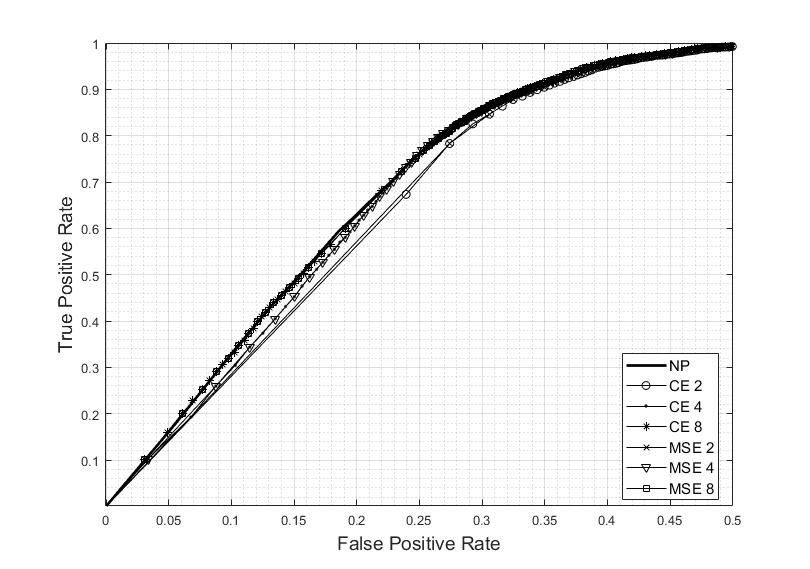
\includegraphics[width=0.5\columnwidth]{mseVSce.jpg}
    \caption{True positive rate vs. false positive rate obtained in the LOS scenario with a single BS. Comparison between NP detector, MLP with MSE training and MLP with CE training with different number of neurons in the hidden layer.}
    \label{fig:ceVSmse}
\end{figure}

Fig. \ref{fig:ceVSmse} show the true positive rate vs. false positive rate obtained by the authentication system with $10^5$ training points and $10^5$ testing points. In particular we here compare the performance of the \ac{np} detector with the \ac{ce}-trained and with the \ac{mse}-trained \acp{mlp}. Furthermore we show the performance of the \acp{mlp} when the hidden layer is composed by $2,4 $ and $8$ neurons. We first notice that the \ac{ce}-trained and \ac{mse}-trained \acp{mlp} obtain the same performance when considering the same number of neurons in the hidden layer. This confirms that the two training methods are performing hypothesis testing in an equivalent manner. Furthermore we notice that as the number of neurons at the hidden layer grows the performance of the \ac{mlp} classificators approach those obtained by the \ac{np} classificator, up to the point where they are the same with $8$ neurons. This shows that both \ac{ce}-trained and \ac{mse}-trained \acp{mlp} are performing the optimal \ac{np} test and that convergence is obtained with a small number of neurons.



\section{Numerical results: non-los scenario}\label{sec:res_nLos}
\subsection{Shadowing effects}\label{sec:shadow}
In this section we consider the non-\ac{los} scenario and we show that the \ac{ml}-based solutions are convenient over the \ac{np}-based one.

Fig. \ref{fig:map} shows a realization of the attenuation map. A spatial grid has been created in order to take into account the shadowing's spatial correlation over different locations in space. The network includes a single \ac{bs} located at the map center and a squared authentic area $\mathcal{A}_0$, delimited in figure by the red line. Furthermore we consider two \ac{los} paths, one parallel to the $x$ axis and one parallel to the $y$ axis and intersecting at the map center.

Consider the \ac{llr} (\ref{eq:lr}). In the non-\ac{los} context the computation of the two area dependent probabilities has no closed-form solution. A numerical solution is obtained by sampling the attenuation values over the spatial grid of positions. Consider an attenuation value $\hat{a}$: the probability of measuring $\hat{a}$ given that the \ac{ue} is located in area $\mathcal{A}_0$ is given by the number of positions $(x_u,y_u)$ inside $\mathcal{A}_0$ where the measured attenuation $a(x_u,y_u)=\hat{a}$ over the total number of positions $(x_u,y_u)$ in the entire map with the same attenuation $\hat{a}$, i.e.
\begin{equation}
    \mathbb{P}(\hat{a}|\mathcal{A}_0) \approx \frac{\text{number of positions} \, (x_u,y_u) \in \mathcal{A}_0 \, \text{s.t.} \, a(x_u,y_u) = \hat{a}}{\text{total number of positions} \, (x_u,y_u) \, \text{s.t.} \, a(x_u,y_u) = \hat{a}}
\end{equation}
An approximation of equation (\ref{eq:lr} is hence obtained as
\begin{equation}\label{eq:lrApp}
    \mathcal{L} \approx \frac{\text{number of positions} \, (x_u,y_u) \in \mathcal{A}_0 \, \text{s.t.} \, a(x_u,y_u) = \hat{a}}{\text{number of positions} \, (x_u,y_u) \in \mathcal{A}_1 \, \text{s.t.} \, a(x_u,y_u) = \hat{a}}
\end{equation}
The approximation gets closer to the real value as the number of grid points over the map increases, as an higher number of points means a better statistical characterization of the attenuation over the map area.

Fig. \ref{fig:trueMap} shows the true positive rate vs. the false positive rate obtained for the attenuation map in Fig. \ref{fig:map}. In particular we here compare the results obtained with approximation (\ref{eq:lrApp}) with the results obtained with the \ac{mse} trained \ac{mlp} with different number of neurons in the hidden layer.
For the computation of (\ref{eq:lrApp}) we built a grid with $4.46 \cdot 10^6$ space points, whereas for training and testing the \ac{mlp} we used respectively $10^5$ and $10^6$ points. We notice that the \ac{mlp} achieves better results than the \ac{np}-based detector. This means that the considered number of grid points is not sufficient to approximate the optimal \ac{np} solution. Furthermore we tested the \ac{mlp} with $1,3$ and $10$ neurons at the hidden layer. We see that the performance with $1$ and $3$ neurons are the same, whereas with $10$ neurons we achieve the \ac{np} solution, based on the results of the previous section. 

Comparing the number of grid points and the number of training points used for the \ac{mlp} we can hence conclude that the \ac{mlp}-based solution is advantageous over the \ac{np}-based one, as it requires a smaller number of points to achieve the optimal solution. Furthermore this implies that the \ac{mlp}-based authentication system can be implemented without a-priory knowledge of the \ac{pdf} of the hypothesis to be tested.

Consider the network in Fig. \ref{fig:mBS}. $N_{\rm bs}=5$ \acp{bs} gather attenuation values from the \acp{ue}. Each \ac{bs} has its own attenuation map given by path loss, shadowing and fading realization. Each \ac{bs} gathers the attenuation value of the transmitting \ac{ue} and sends it to the central unit, which builds the attenuation vector $\bm{a}$ that is used for discriminating the location of the considered \ac{ue}.

Fig. \ref{fig:rnnMLP} compares the performance of the \ac{mlp}-based solution with those of the \ac{rnn}-based solution. Results have been obtained for the network configuration in Fig. \ref{fig:mBS}. Both architectures have been trained over a set of $10^5$ attenuation vectors and tested over the same set of $10^5$ attenuation vectors. Notice that the training set of the \ac{mlp} comprises attenuation vectors measured in both $\mathcal{A}_0$ and $\mathcal{A}_1$. The \ac{mlp} is trained with \ac{mse} loss function and we compare the results obtained with a number of neurons in the hidden layer from $1$ to $5$. The performance of the \ac{rnn}-based solution are here presented for a number of neurons in the hidden layer from $1$ to $5$. Both architectures are composed by an input layer, a hidden layer and an output layer. Curves for the \ac{mlp} are obtained by varying the threshold value $\lambda$, whereas for \ac{rnn} are obtained by varying the threshold value $\gamma$. We notice that the performance of the \ac{rnn} with £4£ neurons in the hidden layer are better compared to those obtained with the \ac{rnn} with $4$ and $5$ neurons in the hidden layer. This is due to the fact that the features extracted by $3$ neurons in the hidden layer better represent data in $\mathcal{A}_0$, whereas $4$ and $5$ neurons are over-representative. This confirms that the feature extraction process of the \ac{rnn} is an efficient way to represent a set. We further notice that the performance of the \ac{rnn} with $2$ neurons in the hidden layer are worse than those obtained with the \ac{rnn} with $3$ neurons in the hidden layer. This is due to the fact that $2$ neurons are not sufficient for the feature extraction process to provide a good characterization of area $\mathcal{A}_0$. We notice that the performance obtained with the \ac{mlp}-solution are better than those obtained with the \ac{rnn}. 

\begin{figure}
    \centering
    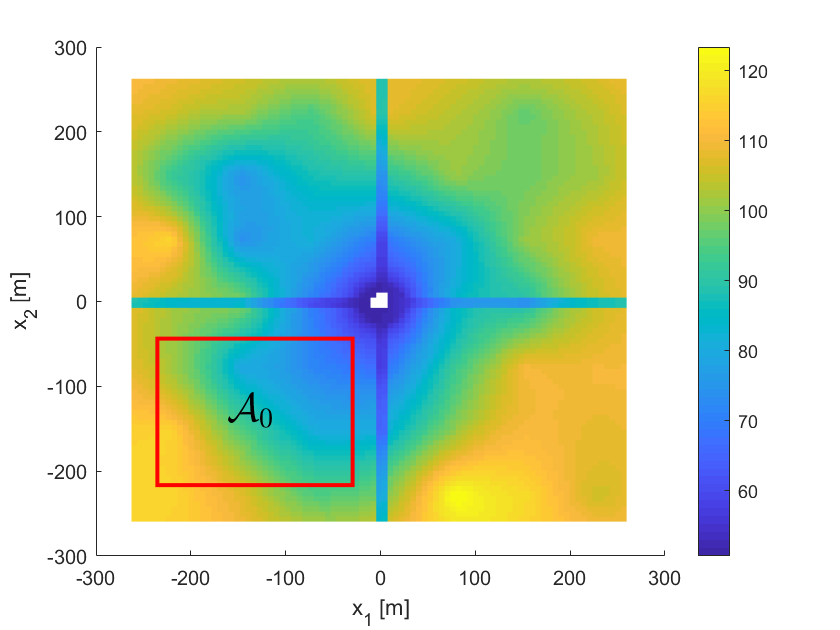
\includegraphics[width=0.5\columnwidth]{surfColorato.png}
    \caption{Example of a realization of the attenuation map in the non-\ac{los} scenario considering only the shadowing effects.}
    \label{fig:map}
\end{figure}


\begin{figure}
    \centering
    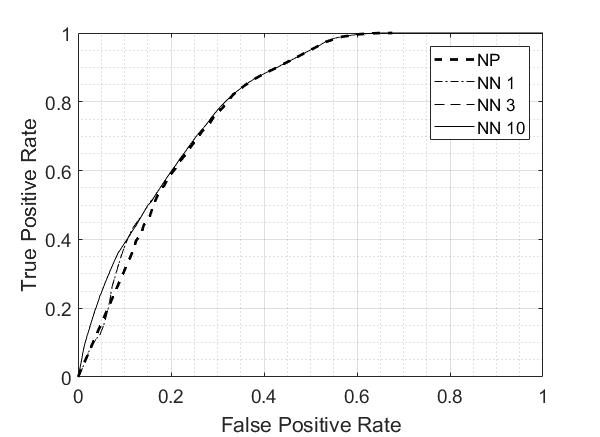
\includegraphics[width=0.5\columnwidth]{trueMap.jpg}
    \caption{True positive rate vs. false positive rate for the attenuation map in Fig. \ref{fig:map}. Comparison between the \ac{np}-based and the \ac{mlp}-based detectors}
    \label{fig:trueMap}
\end{figure}

\begin{figure}
    \centering
    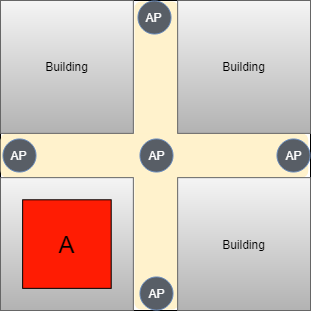
\includegraphics[width=0.3\columnwidth]{scenario2.png}
    \caption{Scenario with multiple BSs: each one gathers the attenuation value of the transmitting user and passes it to the central unit that builds the attenuation vector $\bm{a}$ used for discriminating the location of the user.}
    \label{fig:mBS}
\end{figure}

\begin{figure}
    \centering
    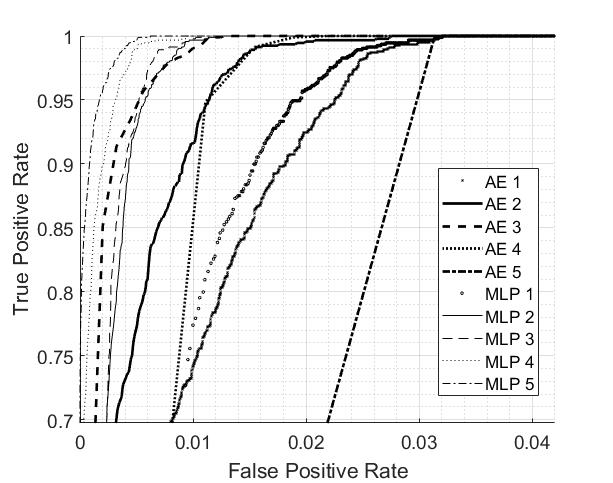
\includegraphics[width=0.5\columnwidth]{RNNvsMLPnNeur.jpg}
    \caption{True positive rate vs. false positive rate for the network configuration in Fig. \ref{fig:mBS}. Comparison between the \ac{mlp}-based and the \ac{rnn}-based detectors with different number of neurons in the hidden layer.}
    \label{fig:rnnMLP}
\end{figure}


\subsection{Fading effects}
Let us now include the fading effects. The attenuation in point $(x_u,y_u)$ is a Gaussian random variable with zero mean and variance given by the inverse of the value of the map in $(x_u,y_u)$.


In order to compute the \ac{llr} in (\ref{eq:lr}) we should here consider a $N_{\rm bs}$-dimensional multivariate Gaussian distribution. However, as this equation has no closed-form solution and we showed in \ref{sec:shadow} that the \ac{mlp}-based solution achieves the optimal results of the \ac{np} detector with fewer points we implement the \ac{mlp}-based solution. A larger number of \acp{bs} means a larger feature space to be fed to the \ac{mlp}. We hence expect that the performance of the system increase with the number of \acp{bs}.

Different fading realizations lead to different statistical characterization of the attenuation values measured in both areas. Therefore training the \ac{mlp} over a single fading realization could lead to a non-optimal result in the successive realization. We hence propose to train and test the \ac{mlp} over $N_{\rm avg}$ fading realizations for each \ac{bs}.

Fig. \ref{fig:faded} shows the true positive rate vs. the false positive rate in non-\ac{los} scenario with fading effects. Different number of fading realizations for training a \ac{mlp} with \ac{mse} loss function has been considered. We notice that as the number $N_{\rm avg}$ of fading realizations used for training increases the performance of the network get closer to those obtained without considering the fading effects. Furthermore we notice that, as expected, with a larger number of \acp{bs} the performance of the system increase, as can be seen comparing the curve in Fig. \ref{fig:trueMap} and the 'No fading' curve in Fig. \ref{fig:faded}.

\begin{figure}
    \centering
    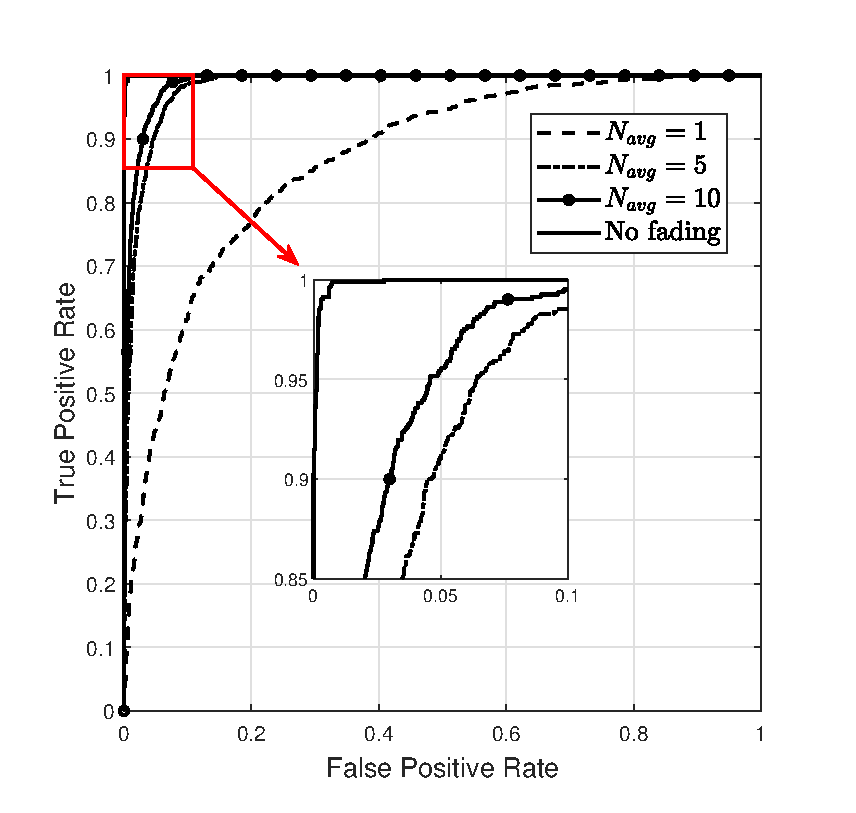
\includegraphics[width=0.5\columnwidth]{Navg.eps}
    \caption{True positive rate vs. false positive rate in non-LOS scenario with fading effects. Comparison between training with different number of fading realizations.}
    \label{fig:faded}
\end{figure}
\newpage 



%\bibliographystyle{IEEEtran}
%\bibliography{bibliography.bib}
\renewcommand*{\bibfont}{\footnotesize}

\printbibliography

\end{document}
